
\textbf{Given:} Consider a $\triangle{ABC}$ with sides AB, BC, AC. Let $\vec{D}$ be the mid-point of AB, $\vec{E}$ be a point on AC and $DE\parallel{BC}$\\
\textbf{Need to prove:} $\vec{E}$ = $ \frac{A+C}{2}$\\
\textbf{Proof:}
\begin{align}
\vec{D} = \frac{A+B}{2} \\
DE\parallel{BC}\label{eq:solutions/1/61}
\end{align}
Let direction vectors be  $\vec{m}_{DE}$ and  $\vec{m}_{BC}$ for line segment DE and BC respectively.
\begin{align}
 \vec{m}_{DE} = \vec{D} - \vec{E} = \frac{\vec{A}+\vec{B}}{2}-\vec{E} \label{eq:solutions/1/62}\\
 \vec{m}_{BC} = \vec{B}-\vec{C}\label{eq:solutions/1/63}
\end{align}
From \eqref{eq:solutions/1/61} we can write the following with $\vec{k}$ being a real value,
\begin{align}
 \vec{m}_{DE} = k \vec{m}_{BC} \label{eq:solutions/1/64}
\end{align} 
Using \eqref{eq:solutions/1/62} and \eqref{eq:solutions/1/63} in the above equation,
\begin{align}
\frac{\vec{A}+\vec{B}}{2}-\vec{E} = k (\vec{B}-\vec{C}) 
%\label{eq:solutions/1/64}
\end{align}
Let $\vec{E} = \frac{m\vec{A}+C}{m+1} \label{eq:solutions/1/65}$ and Substitute $\vec{E}$ in \eqref{eq:solutions/1/64}
\begin{align}
\frac{\vec{A}+\vec{B}}{2}- \frac{m\vec{A}+C}{m+1} = k(\vec{B}-\vec{C})
\end{align}
\begin{align}
\brak{\frac{1}{2}-\frac{m}{m+1}}\vec{A}+\brak{\frac{1}{2}-k}\vec{B}+\brak{k-\frac{1}{m+1}}\vec{C} = 0
\end{align}
Since $\vec{A}$, $\vec{B}$ and $\vec{C}$ are points on a triangle and hence they are Linearly dependent which implies :
\begin{center}
\brak{\frac{1}{2}-\frac{m}{m+1}}=0 and \brak{\frac{1}{2}-k} = 0 and \brak{k-\frac{1}{m+1}} =0 
\end{center}
Therefore we get k = $\frac{1}{2}$ and m = 1.
Substituting m value in $\vec{E}$ we get,
\begin{align}
\vec{E} =  \frac{\vec{A}+\vec{C}}{2}
\end{align} 
\begin{center}
Hence Proved
\end{center}

\begin{figure}[!ht]
\centering
\resizebox{\columnwidth}{!}{
\begin{tikzpicture}

\draw (0,0) node[anchor=north]{$B$}
  -- (4,8) node[anchor=west]{$A$}
  -- (8,0) node[anchor=north]{$C$}
  -- cycle;
\draw (4,0) node[anchor=north]{$E$}
  -- (2,4) node[anchor=east]{$D$}
  -- (6,4) node[anchor=west]{$F$}
  -- cycle;
\end{tikzpicture}

}
%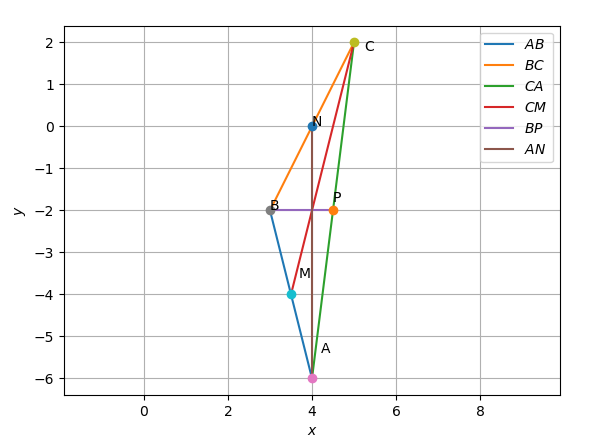
\includegraphics[width=\columnwidth]{./solutions/1/6/triangle.tex}
\caption{Triangle}
\label{fig:Triangle}
\end{figure}
